\documentclass[preprint]{aastex}

\newcommand{\thetitle}{Title of Report}
\newcommand{\theauthor}{Your Name}
\newcommand{\theauthorsemail}{yourname@berkeley.edu}
\newcommand{\thedate}{\today}
% the following controls some aspects of how the text is displayed on the page
\setlength{\textwidth}{6.5in}
\setlength{\textheight}{8.25in}
\setlength{\oddsidemargin}{0in}

% set up the page headers and footers
\usepackage{fancyhdr}
    \pagestyle{fancy}
    \lhead{\sffamily\slshape\small\thetitle}
    \rhead{\sffamily\small\theauthor}
    \cfoot{\sffamily\slshape\small\thepage}

\usepackage{graphicx} % support display of graphics
\usepackage{amsmath,amssymb,latexsym} % import library of technical symbols
\usepackage{natbib} % import bibliography tools

% the following control some aspects of how paragraphs are displayed
\parindent=0pt
\parskip=2ex


\begin{document}
% print the title in san-serif font, in bold, in huge characters
\title{
    \sffamily\bfseries\huge
    \thetitle \\
}
% print the author in san-serif font
\author{
    \sffamily\theauthor \\
    \sffamily\theauthorsemail
}
\begin{abstract}
The abstract is where I give the reader the highlights and spoilers for what is 
contained in this report, including a brief description of what I was seeking 
to explore and what my results were, so that they will know whether or not they 
want to keep reading to get all of the details. The abstract should end with a 
statement of what the conclusions are.  Anyone who has read the abstract of a 
paper should be able to give a quick and accurate summary of what is contained 
within it.
\end{abstract}

\section{Introduction}

In the introduction, we give the context for why this report exists. This 
section generally includes an overview about the current understanding of the 
given topic, what the open questions are, and what this report does to push on 
those boundaries. This is a good place to provide background knowledge to the 
reader, such as important mathematics and fundamental theory that are relevant 
to the report.

For example, if we were giving a report on interferometry, we might want to remind 
my reader what the equation for a visibility is. To include an equation, I 
would do something like this.

\begin{equation}
    \label{eq:vis}
    V(u,v) = \int A(\hat{s}) \cdot I_{sky}(\hat{s}) ~e^{-2 \pi i \frac{\vec{b} 
    \cdot \hat{s}}{\lambda}} d\Omega
\end{equation}

And below, I would follow up by giving definitions for the variables in the 
equation, such as $A(\hat{s})$. I would also be sure to reference this equation 
in the text so that the reader knows why it's important, like this: 
Eq.~\eqref{eq:vis}.

\section{Method}

Here I give a detailed description of what I experimentally observed, including 
information about who performed the experiment, when the experiment took place, 
what equipment was used, how data was recorded, and any particulars or 
peculiarities that might be useful for anyone who may be trying to recreate my 
results.

\section{Results}

In this section, I review the techniques through which I processed and analyzed 
my data, and give the actual results. I also provide the key numbers and data 
that will be fundamental to a reader's understanding of the results. This can 
be a helpful time for a table or a figure, such as 
Fig.~\ref{fig:figure-example}.  I also give some interpretation of what these 
results mean scientifically and for the broader research community, tying back 
into the issues that I mentioned in the introduction!

\begin{figure}
    \begin{center}
    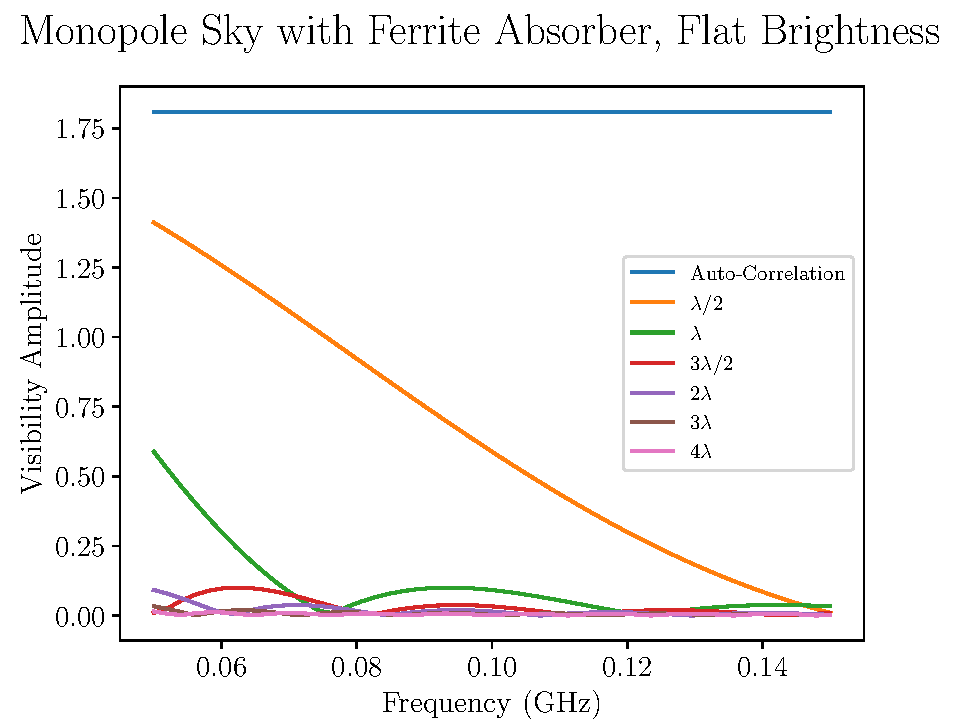
\includegraphics[width=\linewidth]{fig_example}
    \end{center}
    \caption{
        This is a caption describing what is shown in the figure, and 
        describing its relevance and importance to the reader.
    }
    \label{fig:figure-example}
\end{figure}

\section{Conclusions}

Finally, in the conclusion, I review the important points made in the report 
and give a quick summary of the results. I also lay out aspects that are 
lacking in the report, such as known experimental failings or data points that 
need deeper analysis. I describe ways that I could make the experiment better 
and potential future work to follow-up on the results I have found.

 % the following prints the bibliography, the second argument (follows
 % thebibliography) is the longest citation (latex uses it to figure out the
 % spacing in the bibliography). In this case, we are using a number for our
 % citation, and there are less than 10 references, so we just give what I
 % believe is the fastest single digit number, though any digit other than 1
 % would probably work as well.
\begin{thebibliography}{0}
 \bibitem[Name (Year)]{name-year}
  Author Name. \emph{Title of Paper.} Journal Name, volume no., page numbers, 
  publication year.
\end{thebibliography}

\end{document}
